%Copyright (c) 2004 2005 2006 Atos Origin
%Permission is granted to copy, distribute and/or modify this
%document
%under the terms of the GNU Free Documentation License,
%      Version 1.2
%      or any later version published by the Free Software
%      Foundation;
%      with no Invariant Sections, no Front-Cover
%      Texts, and no Back-Cover
%      Texts.  A copy of the license is
%      included in the section entitled "GNU
%      Free Documentation License".
%
% $Id: overview.tex,v 1.4 2006/03/29 14:06:07 goneri Exp $
\documentclass[a4paper]{article}


\usepackage[latin1]{inputenc} % LaTeX, comprends les accents !
\usepackage[T1]{fontenc}      % Police contenant les caract�res fran�ais
\usepackage{geometry}         % D�finir les marges
\usepackage{hyperref}
\usepackage{graphicx}  % picture incusion 
\usepackage{url}
\usepackage{color}
\usepackage{fancyhdr}
\pagestyle{fancy}
\usepackage{float}
%\floatstyle{ruled}
%\newfloat{figure}{thp}{lop}
\newfloat{figure}{!htb}{lop}
\floatname{figure}

\date{Janvier 2006}
\title{Introducing QSOS}
% title param :  title, author, date
\begin{document}

\renewcommand{\footrulewidth}{0.5pt}

\renewcommand{\arraystretch}{1.75} 
\setlength{\tabcolsep}{10pt}

% MACRO
% TabluarStrong : for tabular colonne title
\newcommand{\TS}[1]{\textbf{#1}}

\section{Introducing QSOS}
QSOS is a method, designed to qualify, select and compare free and open source software
in an objective, traceable and argued way.
It publicly available under the terms of the GNU Free Documentation License.

\begin{figure}
\center
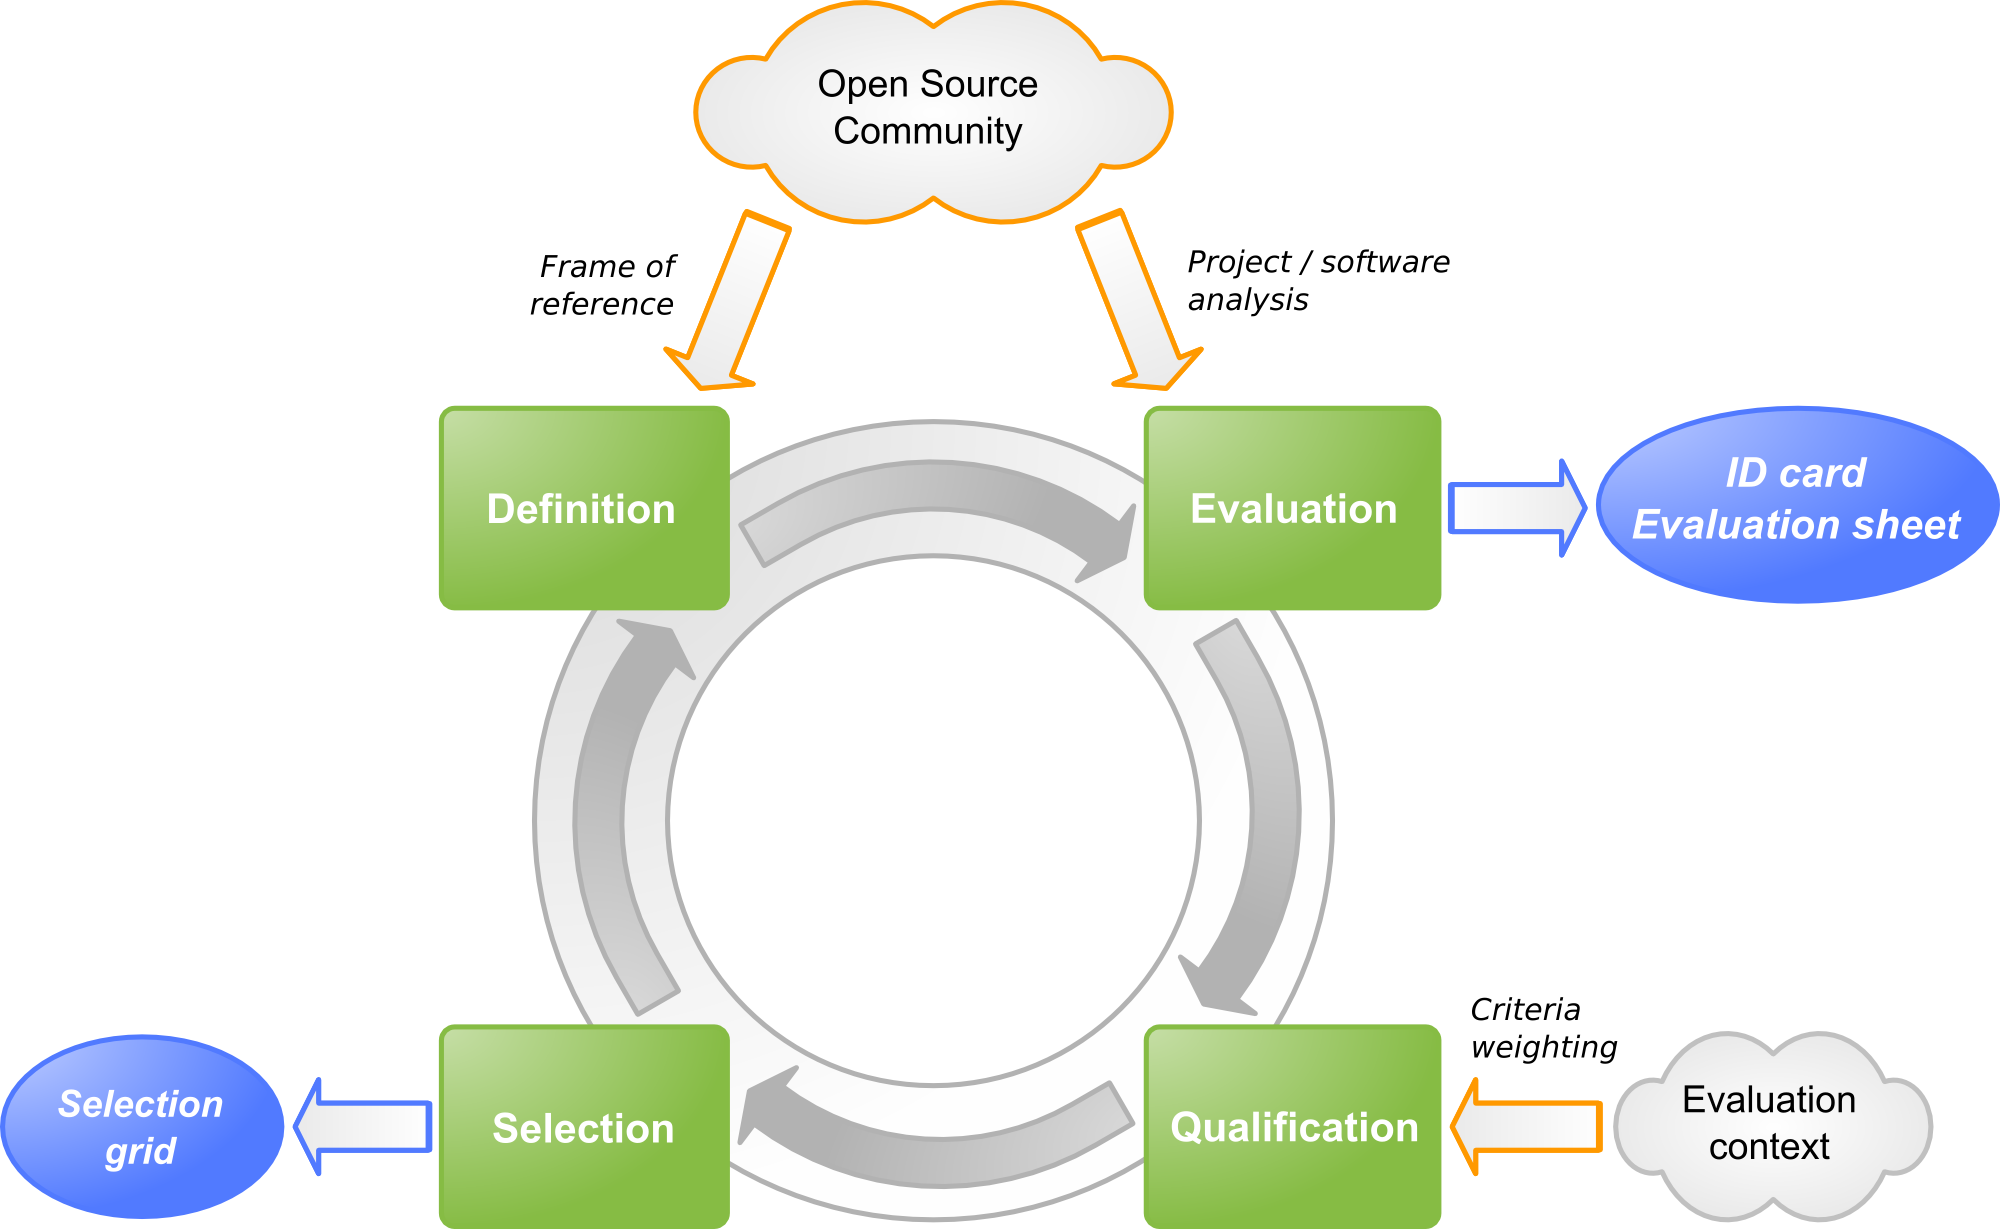
\includegraphics[width=13cm]{images/processus_4_etapes}
\caption{Global process}
\end{figure}


QSOS process is made up of several interdependent and iterative steps:

\begin{itemize}
\item Definition of frames of reference used in the following steps (licenses, 
communities, functional grids by software family, ...).
\item Evaluation of software on three major axis: functional coverage, risks for the
user and risks for the service provider (expertise, training, support services).
Each axis contains several criteria. For instance, the User's risks axis includes:
intrinsic durability, integration, technical adaptability, industrialization
and strategy. These criteria are themselves made up of lower criteria.
\item Qualification of a specific user's context (company or individual) by weighting of 
the previous criteria 
\item Selection and comparison of software fullfilling the requirements.
\end{itemize}


This process generates software ID cards and software evaluation sheets. This
step by step approach, the multiple criteria of analysis and the scoring
model defined by QSOS allow objective and traceable evaluation of free and
open source software. This proves relevant when studying migration opportunity
or when selecting the best open source solution in a given context. 



\end{document}
% vi:syntax=tex
